% document formatting
\documentclass[10pt]{article}
\usepackage[utf8]{inputenc}
\usepackage[left=1in,right=1in,top=1in,bottom=1in]{geometry}
\usepackage[T1]{fontenc}
\usepackage{xcolor}

% math symbols, etc.
\usepackage{amsmath, amsfonts, amssymb, amsthm}

% lists
\usepackage{enumerate}
\usepackage{enumitem}

% images
\usepackage{graphicx} % for images
\usepackage{tikz}

% code blocks
% \usepackage{minted, listings} 

% verbatim greek
\usepackage{alphabeta}

\graphicspath{{./assets/images/Week 6}}

\title{02-614 Week 6 \\ \large{String Algorithms}}
 
\author{Aidan Jan}

\date{\today}

\begin{document}
\maketitle

\section*{An Algorithm to Construct Non-Compressed Suffix Trees (Tries)}
When a suffix tree is built, we read the string in from left to right.  Consider the string $S = abbacabaa$.  For example, when we get to $i = 4$, assume we have a valid suffix tree for the first four characters (i.e., $S_4 = abba$), $T_4$, encoding all the suffixes of $S_4$.  To get to $i = 5$, we will add onto $T_4$ to create $T_5$.
\begin{itemize}
	\item To do this, notice that all the suffixes of $T_4$ are connected by suffix links.  That is, $abba$ has a link to $bba$ which has a link to $ba$, etc.
	\item To append the next character, we start from the deepest node representing the entire string so far, add a new node for the next character, follow the suffix link, and repeat the process until the root is reached.
	\item Update suffix links.
\end{itemize}
This algorithm constructs the Suffix Trie, and runs in quadratic time.

\section*{Ukkonen's Algorithm}
Ukkonen's Algorithm creates a suffix tree (compressed) without the extra nodes.  An ``extra node'' is a node that does not branch, and can therefore be combined into other nodes.
\begin{itemize}
	\item Same basic structure as the previous algorithm
	\item Does not create unnecessary nodes
\end{itemize}
This adds on a new issue: what if we want to extend off of a middle of a node?  Since a node can contain multiple characters now, there will be some cases where a node needs to be converted into a branch.  This introduces multiple cases of adding nodes.\\\\
Suppose the character we want to add is $c$.
\begin{itemize}
	\item \textbf{Case A:} Extending a leaf node.
	\item \textbf{Case B:} Extending an internal node which currently has no child with $c$.
	\item \textbf{Case C:} Extending an internal node which already has an edge for $c$.
	\item \textbf{Case D:} Extending an edge where the next character is $c$.
	\item \textbf{Case E:} Extending an edge where the next character is not $c$.
\end{itemize}

\subsection*{Case A}
We want to extend a leaf node.  (Let red nodes be leaves)
\begin{center}
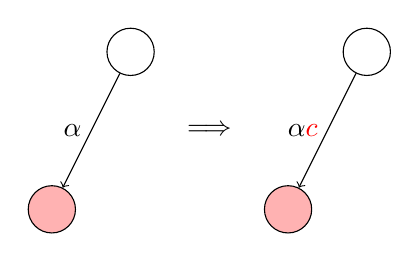
\begin{tikzpicture}
    \node[draw, circle, minimum size=0.6cm] at (0, 0) (r0) {};
    \node[draw, circle, fill=red!30, minimum size=0.6cm] at (-1, -2) (l0) {};
    
    \node at (1, -1) (arrow) {$\Longrightarrow$};

    \node[draw, circle, minimum size=0.6cm] at (3, 0) (r1) {};
    \node[draw, circle, fill=red!30, minimum size=0.6cm] at (2, -2) (l1) {};

    \draw[->] (r0) -- node[left] {$\alpha$} (l0);
    \draw[->] (r1) -- node[left] {$\alpha \textcolor{red}{c}$} (l1);
\end{tikzpicture}
\end{center}
Since there is no new node, there is no new suffix link.

\subsection*{Case B}
Extend an internal node where the node for $c$ does not yet exist.
\begin{center}
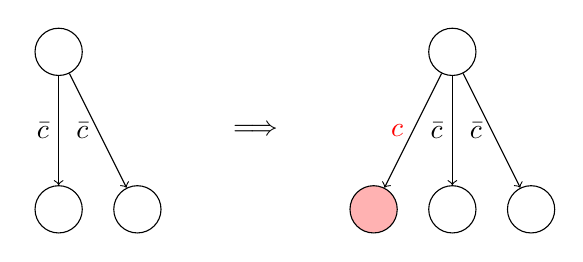
\begin{tikzpicture}
    \node[draw, circle, minimum size=0.6cm] at (0, 0) (r0a) {};
    \node[draw, circle, minimum size=0.6cm] at (0, -2) (l1a) {};
    \node[draw, circle, minimum size=0.6cm] at (1, -2) (l2a) {};
    
    \node at (2.5, -1) (arrow) {$\Longrightarrow$};

    \node[draw, circle, minimum size=0.6cm] at (5, 0) (r0b) {};
    \node[draw, circle, fill=red!30, minimum size=0.6cm] at (4, -2) (l0b) {};
    \node[draw, circle, minimum size=0.6cm] at (5, -2) (l1b) {};
    \node[draw, circle, minimum size=0.6cm] at (6, -2) (l2b) {};

    \draw[->] (r0a) -- node[left] {$\bar{c}$} (l1a);
    \draw[->] (r0a) -- node[left] {$\bar{c}$} (l2a);

    \draw[->] (r0b) -- node[left] {$\textcolor{red}{c}$} (l0b);
    \draw[->] (r0b) -- node[left] {$\bar{c}$} (l1b);
    \draw[->] (r0b) -- node[left] {$\bar{c}$} (l2b);
\end{tikzpicture}
\end{center}
Since a node was added here, it receives a suffix link, pointing to whichever next node when we move up.

\subsection*{Case C}
Extend an internal node where the node for $c$ exists already.
\begin{itemize}
	\item For this case, we do nothing and stop moving backwards through the suffix links.
	\item If the node for $c$ exists already, then we do nothing because it already exists.
	\item We stop moving backwards because if we didn't change the current node, then suffix links won't be updated for any of the parent nodes either.
\end{itemize}

\subsection*{Case D}
Extend an edge where the next character is $c$.
\begin{itemize}
	\item Again, we do nothing for this case and stop moving backwards through the suffix links.
	\item If $c$ exists in an edge, there is no reason to separate it into a new node since branching won't happen anyways.
	\item Moving backwards is also not necessary since because this node (or edge) did not change, the parents won't change either.
\end{itemize}

\pagebreak
\subsection*{Case E}
Extend an edge where the next character is not $c$.
\begin{itemize}
	\item This is the tricky case; we need to break the edge and create a new node in the middle.
\end{itemize}
\begin{center}
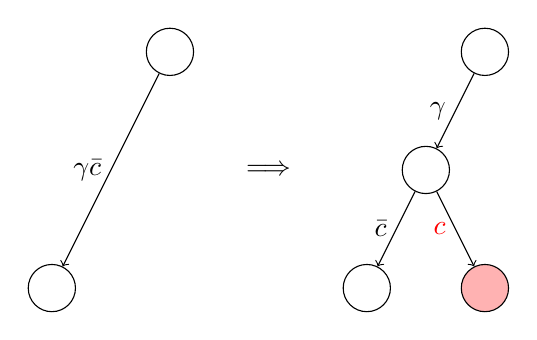
\begin{tikzpicture}
    \node[draw, circle, minimum size=0.6cm] at (0, 0) (r0a) {};
    \node[draw, circle, minimum size=0.6cm] at (-1.5, -3) (l0a) {};
    
    \node at (1.25, -1.5) (arrow) {$\Longrightarrow$};

    \node[draw, circle, minimum size=0.6cm] at (4, 0) (r0b) {};
    \node[draw, circle, minimum size=0.6cm] at (3.25, -1.5) (i1b) {};
    \node[draw, circle, minimum size=0.6cm] at (2.5, -3) (l0b) {};
    \node[draw, circle, fill=red!30, minimum size=0.6cm] at (4, -3) (l1b) {};

    \draw[->] (r0a) -- node[left] {$\gamma\bar{c}$} (l0a);
    
    \draw[->] (r0b) -- node[left] {$\gamma$} (i1b);
    \draw[->] (i1b) -- node[left] {$\bar{c}$} (l0b);
    \draw[->] (i1b) -- node[left] {$\textcolor{red}{c}$} (l1b);
\end{tikzpicture}
\end{center}
For suffix links for case E, when we break an edge and add a node, we lose the suffix link that points to the next location we are supposed to be at.  Depending on where in the edge we added the new node, the suffix link does not exist yet.  We must then take the slow way and traverse the graph downwards from the grandparent's suffix link.
\begin{itemize}
	\item Let each move downwards through the graph be called a \textit{hop}.  Hopping down from the previous node takes $O(|\gamma|)$ time since we have to traverse $|\gamma|$ nodes.
\end{itemize}

\subsection*{Faster Case A}
Recall that suffix trees don't actually store the characters but rather indices in the original string.  
\begin{itemize}
	\item To do case A faster, suppose a leaf node stores indices $x \::\: y$.  
	\item Adding the current letter gives $x \::\: y + 1$ instead.  However, $y + 1$ is always the length of the string we are currently considering.
	\item To improve the running time, we can instead store a pointer at the leaf nodes, basically $x \::\: \texttt{[int* l]}$, where \texttt{l} is a pointer to the length of the string we are currently considering.
	\item By doing this, we can update all the affected leaf nodes at the same time by just changing the length.
\end{itemize}

\subsection*{Where to Start a Phase}
Let a \textit{phase} be defined as a traversal from the deepest node going up the suffix links, updating the nodes with the current letter.  Essentially, adding one letter to the tree.
\begin{itemize}
	\item Suppose in the current phase, we are adding $A$ to the tree as the next character, and the nodes we traverse have the following characters (in order): $AAAANNANANNX$.  The first character is the deepest leaf node, the $N$'s are characters that are not $A$ that we add nodes to (i.e., cases B and E), and $X$ is either case $C$ or $D$ where we stop traversal.
	\item By the next phase, the same string would look like $AAAAAAAAAAAX$.  This is because we just added $A$, so every node on the suffix link frontier must be $A$.
	\item We can start the next phase at the place we stopped last time if we add the same letter again.  (All the A's now are leaves and are updated automatically with the length.)
\end{itemize}

\subsection*{Runtime}
Note that all of the individual cases take constant time except for case E.  
\begin{itemize}
	\item Cases A - D are all just some local surgery.
	\item Case E is $O(\text{number of hops})$.
\end{itemize}

\subsubsection*{Theorem}
Running time is $O(|\Gamma| + \text{\# hops})$.\\\\
For this to be linear in terms of the string, we need to show that the number of hops in total for the entire string is $O(|T|)$.  We first need to prove this.

\subsubsection*{Lemma:}
The number of hops is $O(|T|)$.\\\\
\textbf{Proof:}
First, note that following a suffix link reduces the node depth by at most 1.  Consider a generic branching path:
\begin{center}
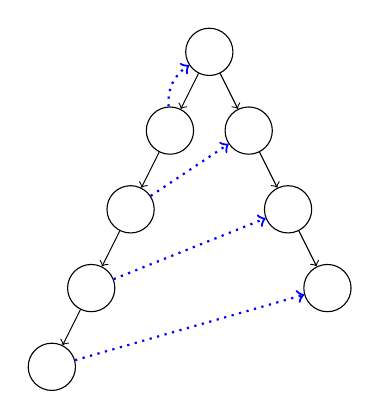
\begin{tikzpicture}
    \node[draw, circle, minimum size=0.6cm] at (0, 0) (root) {};
    \node[draw, circle, minimum size=0.6cm] at (-0.5, -1) (l1) {};
    \node[draw, circle, minimum size=0.6cm] at (-1, -2) (l2) {};
    \node[draw, circle, minimum size=0.6cm] at (-1.5, -3) (l3) {};
    \node[draw, circle, minimum size=0.6cm] at (-2, -4) (l4) {};
    \node[draw, circle, minimum size=0.6cm] at (0.5, -1) (r1) {};
    \node[draw, circle, minimum size=0.6cm] at (1, -2) (r2) {};
    \node[draw, circle, minimum size=0.6cm] at (1.5, -3) (r3) {};

    % edges
    \draw[->] (root) -- (l1);
    \draw[->] (l1) -- (l2);
    \draw[->] (l2) -- (l3);
    \draw[->] (l3) -- (l4);
    \draw[->] (root) -- (r1);
    \draw[->] (r1) -- (r2);
    \draw[->] (r2) -- (r3);

    % suffix links
    \draw[->, blue, dotted, thick] (l4) -- (r3);
    \draw[->, blue, dotted, thick] (l3) -- (r2);
    \draw[->, blue, dotted, thick] (l2) -- (r1);
    \draw[->, blue, dotted, thick] (l1) to[bend left] (root);
\end{tikzpicture}
\end{center}
By the way suffix links are defined, links from the left branch in this case must point to those on other branch(es).  Additionally, suffix links should be ``parallel'' in that two nodes linked by suffix links would mean their parents are also linked by suffix links.  Thus, at most one node on the longer branch can point to the root; the others will be paired up as shown above.\\\\
As a consequence, if we break an edge and add a node in the middle, the most we will have to backtrack would be just the number of characters the edge represents, which must be linear.\\
\rule{\textwidth}{1pt}
If $\Phi :=$ the current \textit{node} depth, then
\begin{align*}
    \Phi_{\text{final}} &\geq 0 + \sum_{\text{operation }i} (\text{hops}_i - 2) \geq \text{hops} - 4|T| \\
    |T| &\geq \Phi_{\text{final}} \geq \text{hops} - 4|T| \\
    \Rightarrow 5|T| &\geq \text{\#hops}
\end{align*}





\end{document}